\subsection{Interval estimate}
\label{sec:etas-interval}


Deciding on a ``best'' single-value estimate of arrival time is exceedingly difficult given the amount of uncertainty involved. The best approach above is to use a small quantile, but this increases expected wait time given catching the bus (top-right of \cref{fig:eta_headway_results}). An alternative approach is to provide \emph{two} estimates---a lower and upper bound---that is to say, a \emph{prediction interval}. Such an interval should be both \emph{reliable} and \emph{useful} for commuters.

Reliability means that, if one arrives by the \emph{lower estimate}, there is only a small probability of missing the bus. The bus should also have a low chance of arriving after the \emph{upper estimate}, particularly when using the prediction to decide which bus to catch to get to a destination on time (more of this in \cref{sec:etas-journey-planning}).

Usefulness corresponds to the interval's width and expected wait time. These should both be minimised where possible, so for example, if a bus is 5~minutes away, providing a 30-minute interval should only be done if there is a valid reason to do so. If there is a layover between the bus and the passenger's stop, for example, the time range could very well be that large since the particles implement the layover behaviour discussed in \cref{sec:prediction_arrival_time}.







Here we consider symmetric $100(1-\alpha)$\% prediction intervals, $\alpha\in (0,1)$, of the form
\begin{equation}
\left(\hat\Teta_{\alpha/2},\ \hat\Teta_{1-\alpha/2}+1\right),
\end{equation}
where $\hat A_q$ is as defined in \cref{eq:eta_calc_quantile}. The ``plus one'' is used to ensure the probability of the bus arriving before the upper bound is \emph{at least} $1-\frac{\alpha}{2}$. Note that although these intervals are symmetric in probability, they are most often asymmetric on the arrival time scale, particularly when the bus is near and the distribution is right-skewed, as shown in \cref{fig:eta_dist_skew}. In contrast, a Kalman filter implementation assumes Gaussian errors, so a symmetric interval ($y$-axis) is also symmetric around the mean ($x$-axis), as shown, often leading to incorrect intervals (potentially even an \gls{eta} below zero).


\begin{knitrout}\small
\definecolor{shadecolor}{rgb}{0.969, 0.969, 0.969}\color{fgcolor}\begin{figure}

{\centering 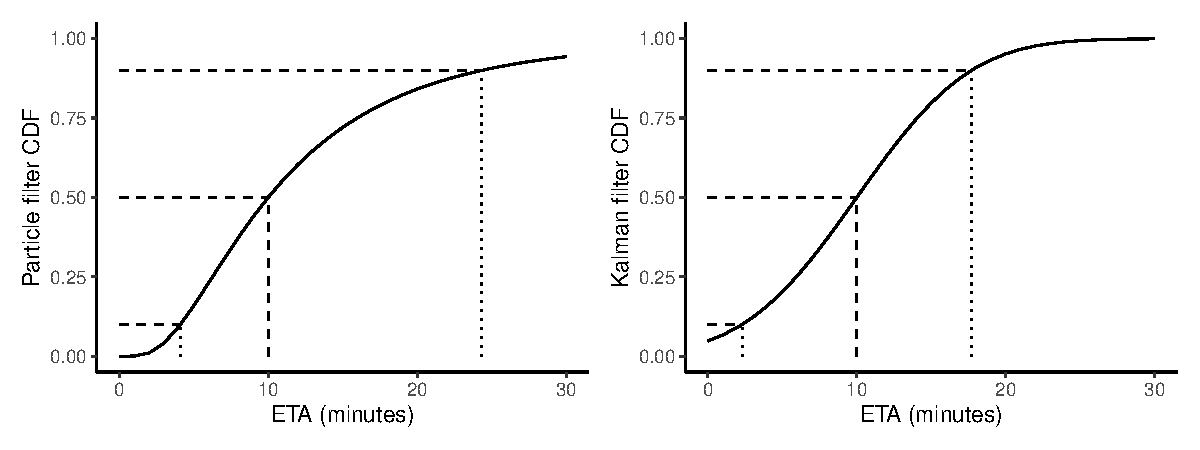
\includegraphics[width=\textwidth]{figure/eta_dist_skew-1} 

}

\caption[Symmetry of arrival time prediction intervals]{Symmetry of arrival time prediction intervals. Symmetric intervals on the probabilty scale map to asymmetric intervals on the arrival time scale under the particle filter (left), and symmetric intervals on the arrival time scale under the Kalman filter (right).}\label{fig:eta_dist_skew}
\end{figure}


\end{knitrout}


\begin{knitrout}\small
\definecolor{shadecolor}{rgb}{0.969, 0.969, 0.969}\color{fgcolor}\begin{figure}

{\centering 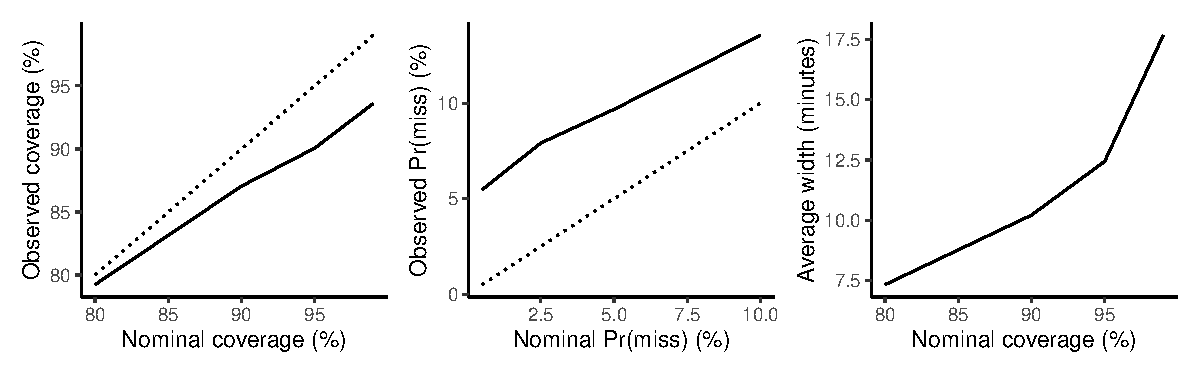
\includegraphics[width=\textwidth]{figure/eta_cis-1} 

}

\caption[Evaluation of prediction intervals from the particle filter arrival time CDF]{Evaluation of the observed coverage (left), lower bound (middle), and width (right) of various prediction intervals using the particle filter arrival time CDF. The dotted line indicates the nominal value.}\label{fig:eta_cis}
\end{figure}


\end{knitrout}



I computed intervals for $\alpha \in \{0.01, 0.05, 0.1, 0.2\}$, and for each evaluated the observed coverage, the proportion of times that the bus arrived before the lower bound, and the average interval width (in minutes). \Cref{fig:eta_cis} shows that the observed coverage drops slightly as the interval width increases (smaller $\alpha$) and that the probability of the bus arriving before the lower bound is higher than expected. This may indicate that not enough uncertainty is being incorporated; referring back to \cref{cha:prediction}, much of this occurs during peak times. Interval width increases with coverage probability, demonstrating the trade-off between reliability and usefulness.


Other variables---time-until-arrival, time of day, or stop sequence---are not considered here as in the previous chapter since the results are much the same. However, if desired, such relationships could be explored to choose the best point or interval estimate under any given situation. The goal of this section was to demonstrate that reliability and usefulness can be improved upon by using prediction intervals.
